%======================================================================
\chapter{Hybrid Remote Rendering}
\label{chap:hrr}
%======================================================================

\section{Method}

We propose a remote rendering system that minimizes the network bandwidth requirements and the network latency in remote rendering.
Our approach is a client-server architecture and maintains two versions of models: low-fidelity models and high-fidelity models.
Low and high fidelity models differ in the number of polygons and in rendering quality.

On the client side, the mobile device renders low-fidelity models that have less polygons, lower fidelity of textures and lower quality rendering effects, while on the server side, the workstation renders high-fidelity models that have more polygons, higher fidelity of textures and higher quality rendering effects. Hence key models are rendered on the server and captured in images which are sent to the client as a video stream. We define key models as those that are important to the application. The models that the user is interacting with can be identified from interaction information sent to the server, while the models that are important to the application are specified in advance by the application developers.

This architecture is able to reduce required network bandwidth and latency in user interactions.
Since only the regions of interest of the entire frame are encoded and streamed to the clients, while the rest is discarded, it reduces the bit rate of the encoded video stream.
The user interaction latency is composed of three components: rendering, encoding and network transmission. Our proposed method aims at reducing the rendering time by only rendering and encoding the key models in high-fidelity mode and rendering the rest in low-fidelity mode without encoding.

\subsection{Client-Server Prototype Design}

The proposed system aims at providing high-quality rendering on less powerful mobile devices, while minimizing the amount of data transferred via network.
Moreover, it also needs to enable multi-client cooperation to enhance the user experience in training scenarios.

The proposed system is inspired by Levoy~\cite{levoy1995}, Lamberti and Sanna~\cite{lamberti2007} and Lu et al.~\cite{lu2011}.
It is a hybrid approach of model-based and image-based methods.
On one hand, the low-fidelity models are stored on the client-side and the local rendering capacity is leveraged to produce decent rendering results.
On the other hand, the high-fidelity rendering results of specific models that are required are sent from the server to the client and overlaid upon the locally rendered frames.
In this way, the data transfered via network is minimized since the existence of local models and the pixels sent via the network are restricted at the models that are required by the client.

There are three challenges in realizing a multi-client cooperation system with the functionalities described above.
First, the existence of multiple clients requires that the server must not be blocked by any of the clients.
Second, each client has a different view from all the other clients. This can result in performance issue since a scene needs to be rendered multiple times in one iteration.
Third, because only a subset of the models are rendered on and rent from the server, the occlusion becomes a problem since the model that is closer to the camera might not be required to render.

We address the first problem by interact with each client independently. More specifically, we enable the server to receive interactions from and send them to every client independently, so that if a client becomes unresponsive, the server is not blocked.
The second issue is relieved by implementing the server as "render-on-demand", which means the server renders the scene for a client only when it requires a new frame.
We address the third challenge by a two-pass rendering process. In the first pass, the entire scene is rendered. Then the colour buffer is cleared before the second pass. In this way, the second pass is rendered upon the depth information obtained from the first pass.

As depicted in Fig.~\ref{fig:architecture}, in this system, all clients are connected to the rendering server and send interaction commands to the server.
On the server side, the application status changes according to the commands received from all clients. The application status changes are synchronized with all clients. In this way, the clients are able to cooperate with each other. In other words, when a client changes the status of the application, all clients will see the change immediately.
To minimize the amount of transferred data, the client decides which models need to be rendered in high-fidelity and the server only sends the pixels of those models. The other models are still rendered locally.

Fig.~\ref{fig:swf} illustrates the workflow of communication between the server and the clients. It shows the workloads during one frame on the server and the clients. If the user interaction sent from any client would influence the simulation states of the server, it synchronizes the state changes among all clients, which ensures all clients have the same states. Moreover, the server renders and encodes the frames for all the clients. Upon receiving the high-fidelity frame, the client encodes and overlays it on the locally rendered frame.

\begin{figure}[!htbp]
	\centering
	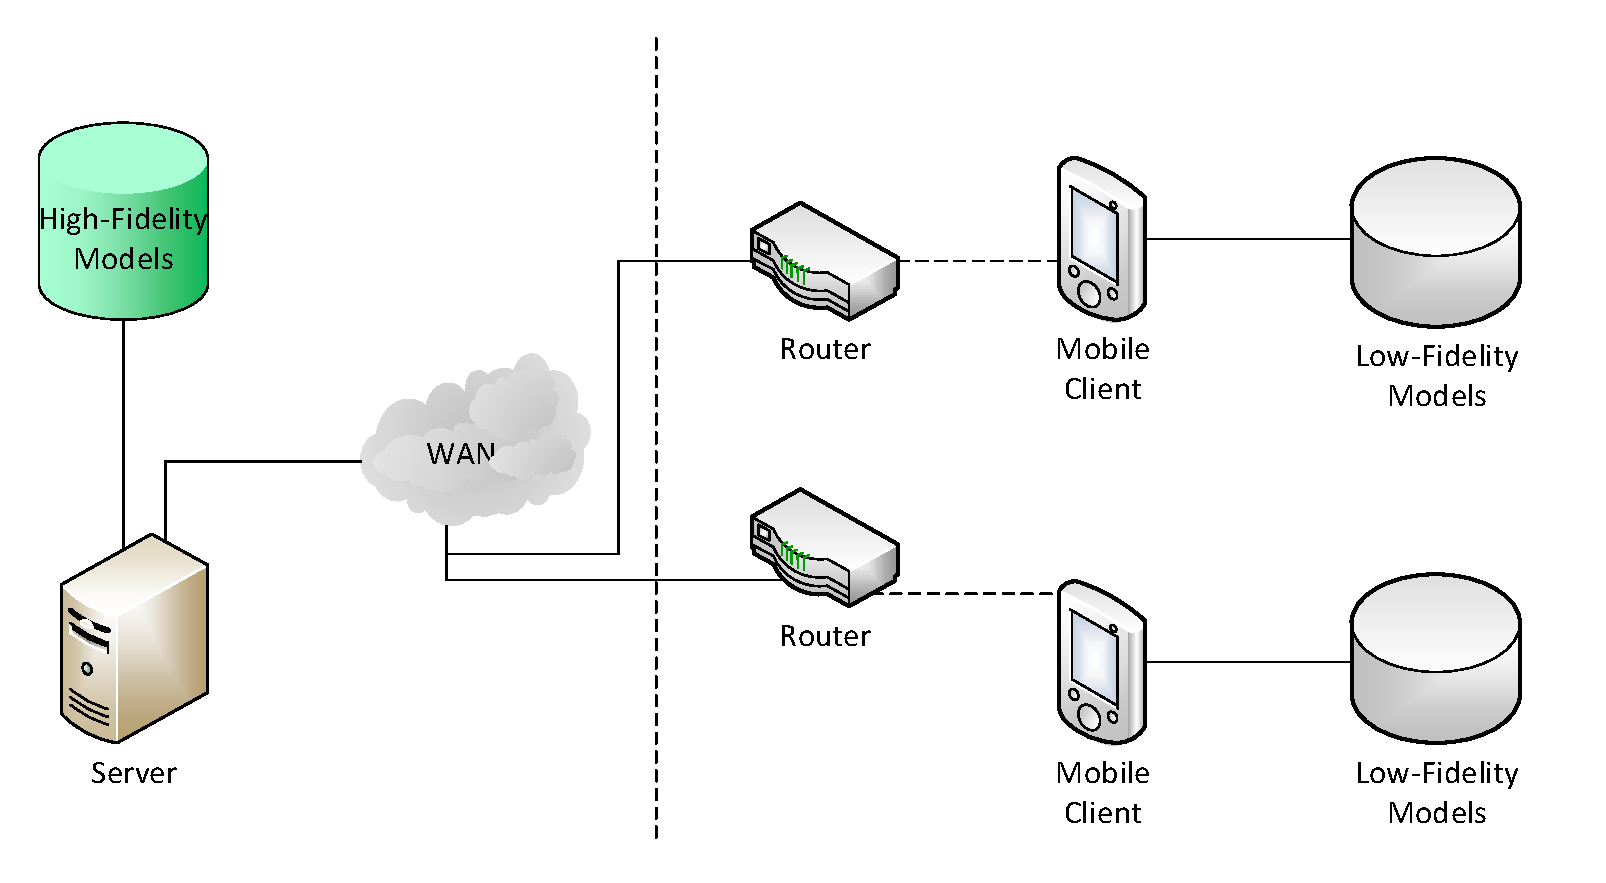
\includegraphics[width=\columnwidth]{figures/architecture.pdf}
	\caption{System architecture}
	\label{fig:architecture}
\end{figure}

\begin{figure}[!htbp]
	\centering
	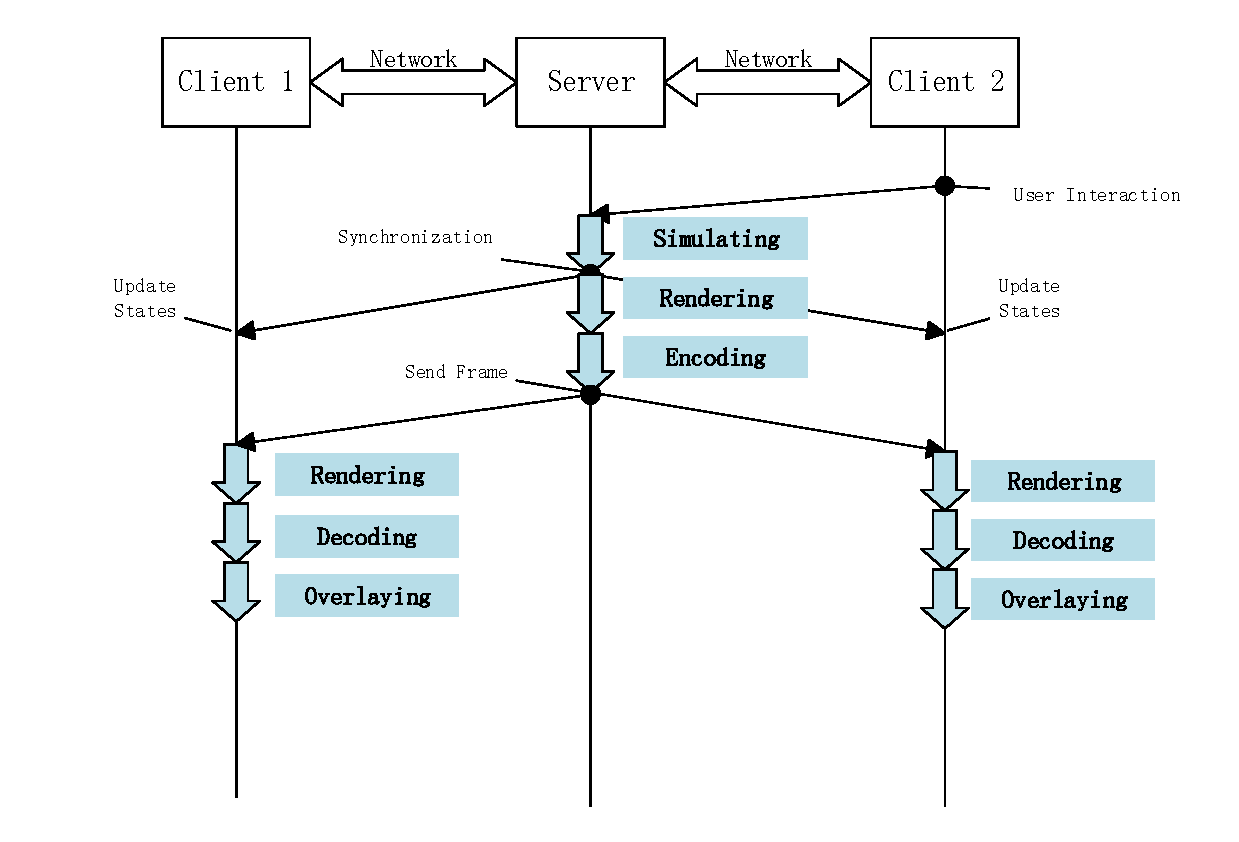
\includegraphics[width=\columnwidth]{figures/sequence_workflow.pdf}
	\caption{Workflow of communication between the server and the clients}
	\label{fig:swf}
\end{figure}

\subsection{Workflows}

Our prototype consists of one server and multiple clients, we will show the workflow of both and various issues in the next sub-sections.
Fig.~\ref{fig:s-wf} shows the workflow of the server.
In each loop, the server updates the simulation status of the scene and receive commands from all clients.
After that, the server sends commands to all clients in order to keep the simulation statuses of those client synchronized.
In the server side, each client has its own view that is independent from all the other clients.
When rendering the scene, the server does not render it for each client, instead, it only renders for the clients that have requested a new frame.

Fig.~\ref{fig:c-wf} indicates the workflow of clients. In each loop, the client gets commands from the server and adjusts the simulation status according to those commands. Then it sends user interaction commands to the server. In each iteration, the client will receive the high-fidelity frame from the server since it has requested in the previous iteration. The client has simplified models stored locally, it renders the scene in every iteration. The high-fidelity frames acquired from the server are overlaid upon the locally rendered frames. Once done, it sends the frame request to the server. In this way, the server does not need to render frames for all clients in every loop, instead it renders a frame when it is needed.

\begin{figure}[!htbp]
	\centering
	\includegraphics[width=0.7\columnwidth]{figures/workflow_server.eps}
	\caption{Server-side Workflow}
	\label{fig:s-wf}
\end{figure}

\begin{figure}[!htbp]
	\centering
	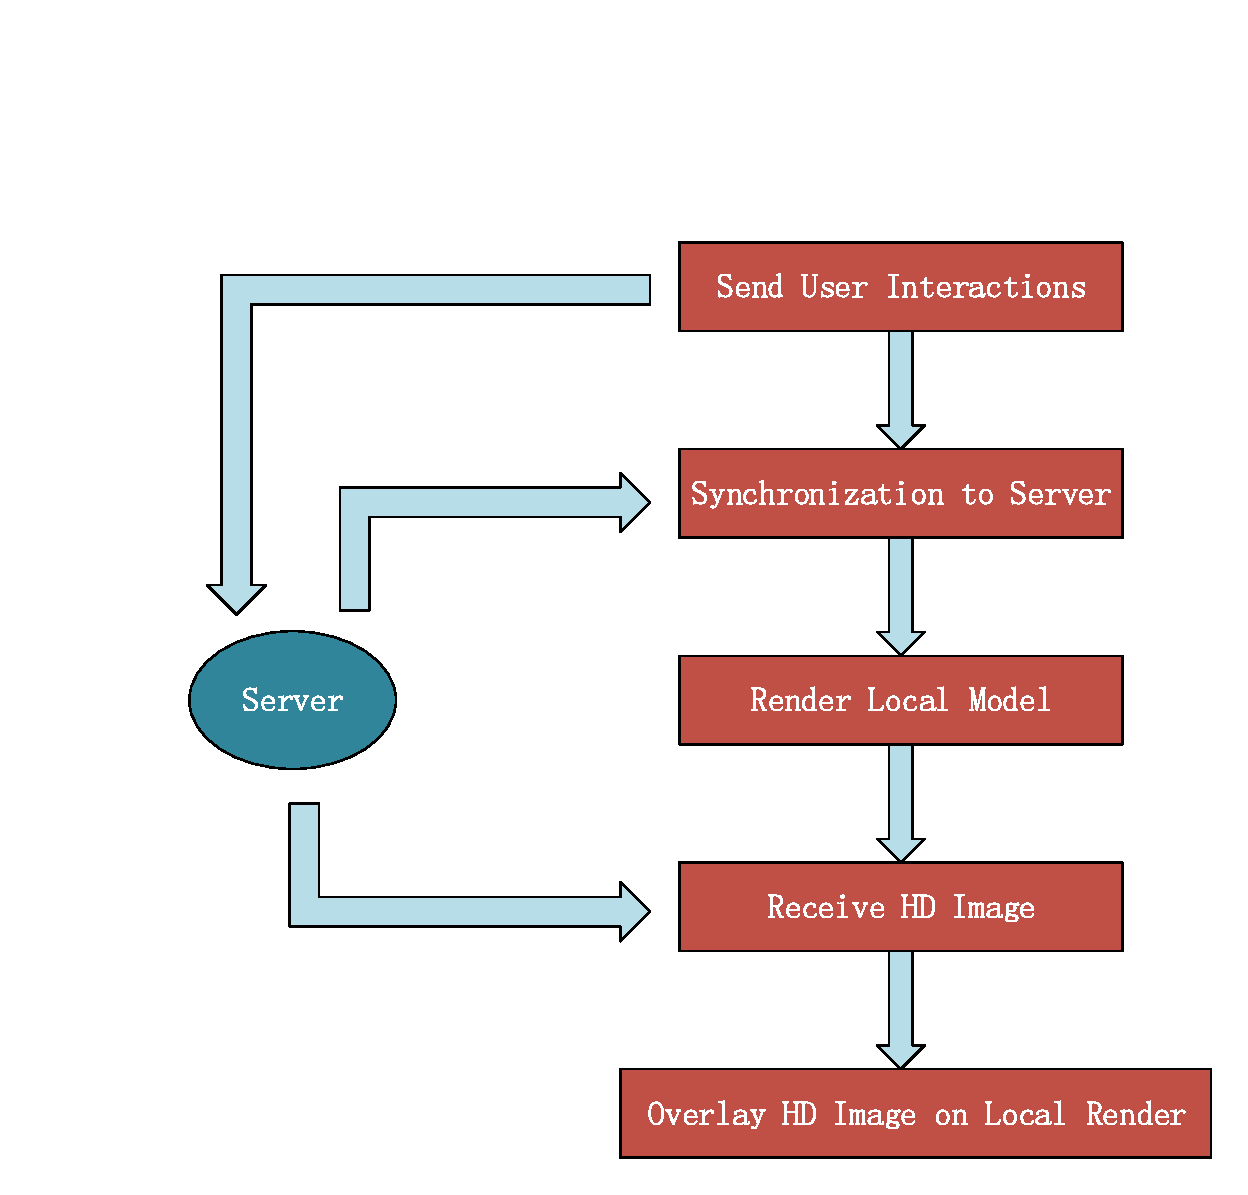
\includegraphics[width=0.7\columnwidth]{figures/workflow_client.pdf}
	\caption{Client-side Workflow}
	\label{fig:c-wf}
\end{figure}

\subsection{Two-pass Rendering}

As mentioned in section \ref{sec:intro}, we use a two-pass rendering processing on the server side.
Because frames sent to the client side contain only the key models, the server renders the high-fidelity version of those key models only.
But this is not enough, since the rest models may occlude the key models.
We propose a two-pass rendering process to address this issue.

\begin{figure}[!htbp]
	\centering
	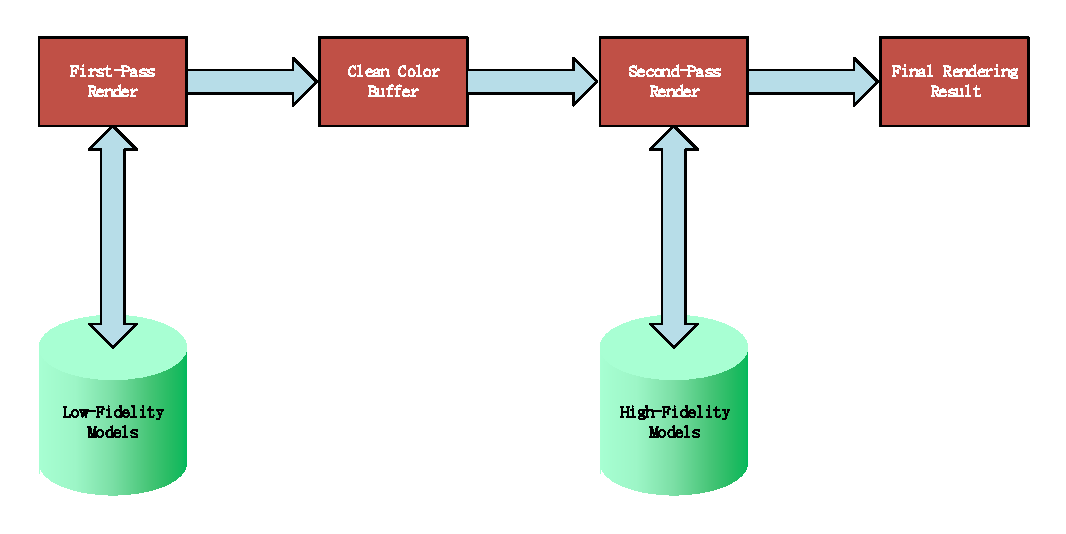
\includegraphics[width=0.7\columnwidth]{figures/two-pass-rendering.pdf}
	\caption{Two-pass rendering}
	\label{fig:tp-rendering}
\end{figure}

As shown in Fig.~\ref{fig:tp-rendering}, in the first pass, it renders all models except for the key models using low-fidelity version of models. Then the color buffer is cleaned and only depth information is preserved. In the second pass, only key models of their high-fidelity version are rendered, while considering the depth information obtained from the first pass rendering, therefore the occlusions are preserved in the final rendering result.

\section{User Study}

In order to validate the use case of our proposed hybrid remote rendering technique, we designed a user study. The user study is contemplated into two parts: a) pre-trial study, b) main study. We conduct and analyze the pre-trial study before the main study.

\subsection{Pre-Trial Study}

In the main study, we vary the model resolution and test its effect on users' ability of object recognition.
It requires a very careful selection of low-level display of the meshes. We would like to therefore to first run a simplified version of the experimental procedure to determine the correct level. We would like to show the participant the same three types of models but rather than the models appearing randomly at different resolutions, the same model would be shown continuously at increasing level of details where at each level, the participant would select the type of the model (dog, cat or horse). In this way we would be able to determine the level at which participants can reliably detect the type of model.

\subsection{Main Study}

In this user study, we aim at validating the Quality of Experience (QoE) improvements that can be achieved by the adoption of the proposed framework for mobile device 3D graphics applications. We use a 3D mobile application that prompts the user to respond rapidly to a visual stimulus in our evaluation. This is a stand in for a variety of applications that require the user to react swiftly to changing aspects in a 3D environment. Examples of such applications are games, flight simulators, military training systems, etc... We compare our results to conventional remote rendering and local rendering approaches.

The test application we use in our experiments depicts one or more 3D objects appearing randomly within a virtual room and disappearing within a short period.  There are 3 types of objects: dogs, cats and horses. For each type, we prepared 5 different 3D models. When the participant sees an object, he/she needs to press on the object and one of three buttons that corresponds to that object, as shown in Fig.~\ref{fig:us}.

\begin{figure}[!htbp]
	\centering
	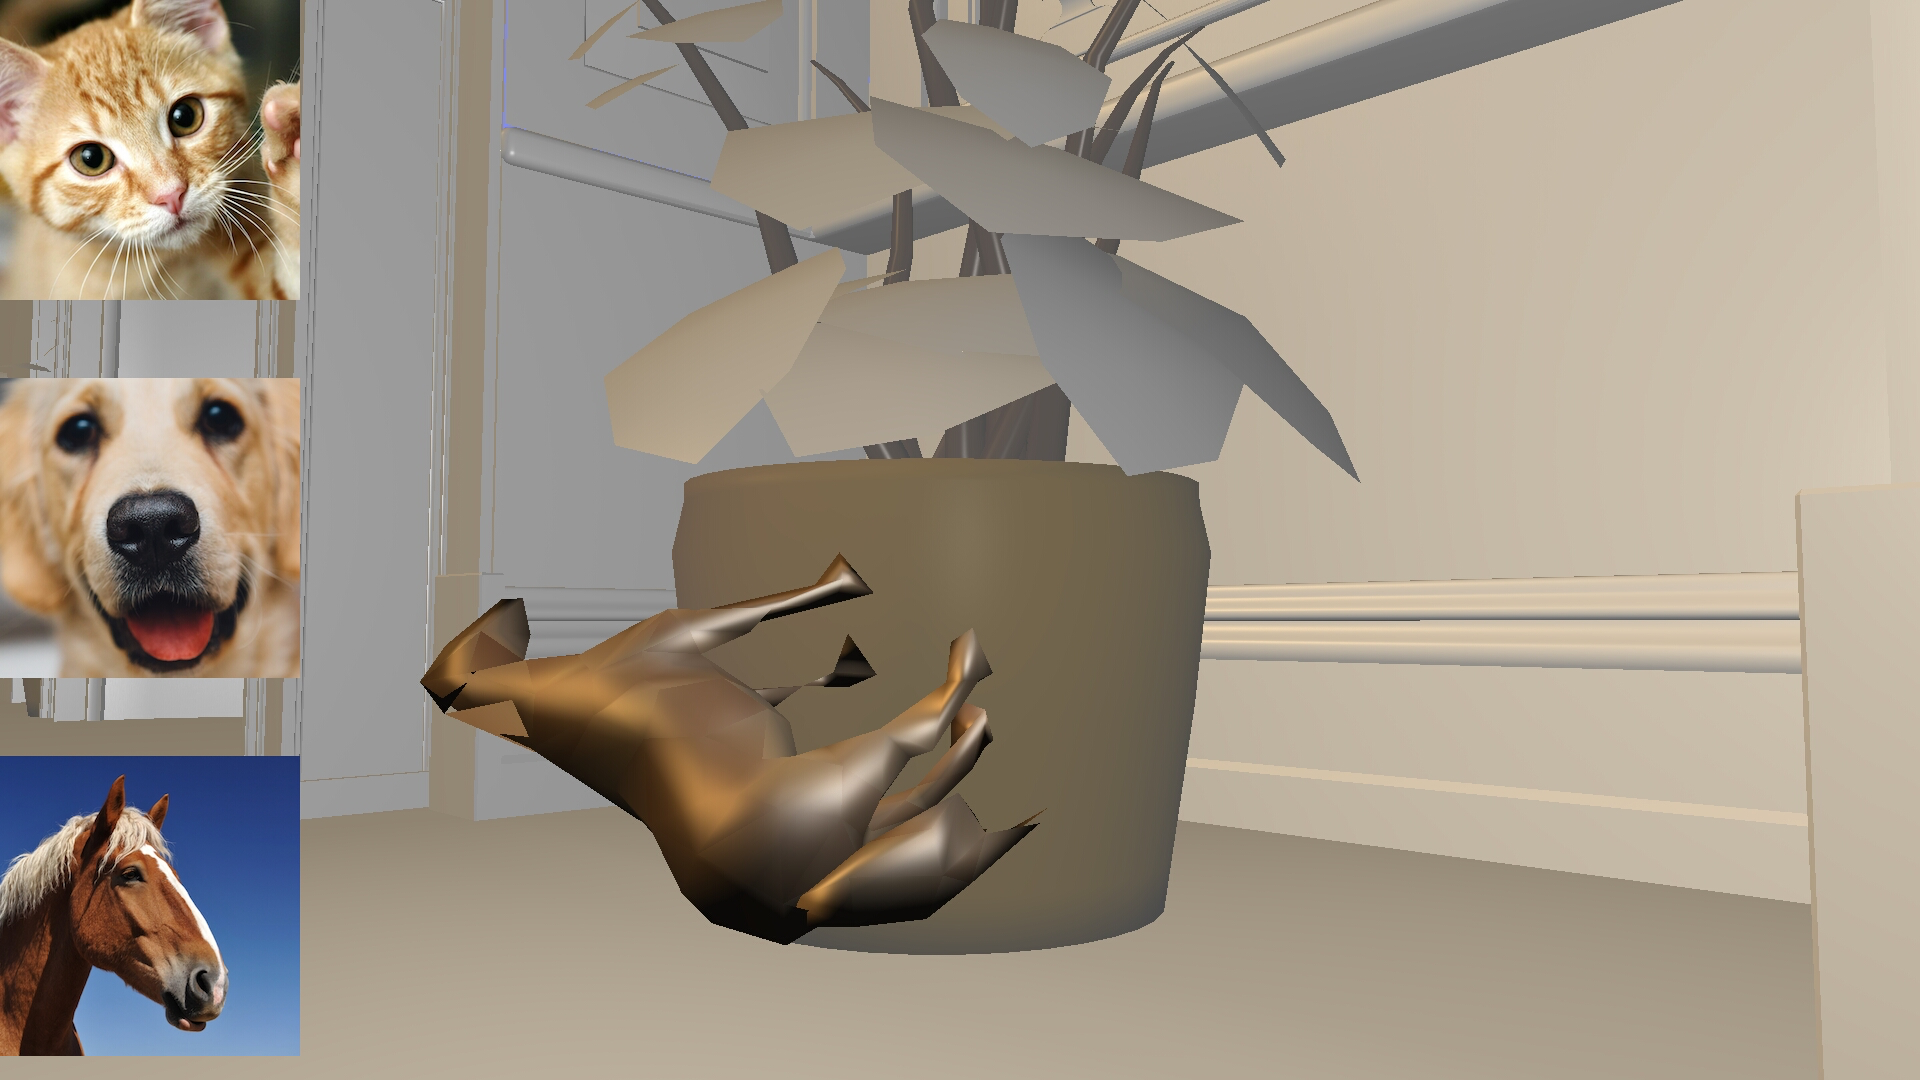
\includegraphics[width=\columnwidth]{figures/user_study.png}
	\caption{Screenshot of the user study application.}
	\label{fig:us}
\end{figure}

We run the test application 20 times for each subject. We vary the model resolution, environment resolution, delay and  jitter across these runs. The table below details the test application configuration for the 20 runs. The order of the 20 configurations will be randomized across subjects to avoid biasing the results.

\begin{table}
\renewcommand{\arraystretch}{1.3}
\caption{Configurations of the main user study application.}
\label{tab:pus}
\centering
\begin{tabular}{|c|c|c|c|c|}
\specialrule{1pt}{0pt}{0pt}
Name & Model Res & Environment Res & Delay & Jitter \\\specialrule{1pt}{0pt}{0pt}
APP\_1 & low & low & $0ms$ & No \\\specialrule{1pt}{0pt}{0pt}
APP\_2 & low & high & $0ms$ & No \\\specialrule{1pt}{0pt}{0pt}
APP\_3 & high & low & $0ms$ & No \\\specialrule{1pt}{0pt}{0pt}
APP\_4 & high & high & $0ms$ & No \\\specialrule{1pt}{0pt}{0pt}
APP\_5 & low & low & $80ms$ & No \\\specialrule{1pt}{0pt}{0pt}
APP\_6 & low & high & $80ms$ & No \\\specialrule{1pt}{0pt}{0pt}
APP\_7 & high & low & $80ms$ & No \\\specialrule{1pt}{0pt}{0pt}
APP\_8 & high & high & $80ms$ & No \\\specialrule{1pt}{0pt}{0pt}
APP\_9 & low & low & $80ms$ & Yes \\\specialrule{1pt}{0pt}{0pt}
APP\_10 & low & high & $80ms$ & Yes \\\specialrule{1pt}{0pt}{0pt}
APP\_11 & high & low & $80ms$ & Yes \\\specialrule{1pt}{0pt}{0pt}
APP\_12 & high & high & $80ms$ & Yes \\\specialrule{1pt}{0pt}{0pt}
APP\_13 & low & low & $120ms$ & No \\\specialrule{1pt}{0pt}{0pt}
APP\_14 & low & high & $120ms$ & No \\\specialrule{1pt}{0pt}{0pt}
APP\_15 & high & low & $120ms$ & No \\\specialrule{1pt}{0pt}{0pt}
APP\_16 & high & high & $120ms$ & No \\\specialrule{1pt}{0pt}{0pt}
APP\_17 & low & low & $120ms$ & Yes \\\specialrule{1pt}{0pt}{0pt}
APP\_18 & low & high & $120ms$ & Yes \\\specialrule{1pt}{0pt}{0pt}
APP\_19 & high & low & $120ms$ & Yes \\\specialrule{1pt}{0pt}{0pt}
APP\_20 & high & high & $120ms$ & Yes \\\specialrule{1pt}{0pt}{0pt}
\end{tabular}
\end{table}

As shown in Tab.~\ref{tab:pus}, we prepare four types of scenes: a scene with only low-resolution models and low-resolution environment, a scene with low-resolution models and high-resolution environment, a scene with high-resolution models and low-resolution environment and a scene with high-resolution models and high-resolution environment.  We simulate three different network delays: $0ms$, $80ms$ and $120ms$. We also consider network jitter, where network jitter is the sudden fluctuation on the network.

As the user interacts with the test application, we collect two types of data: QoE and user performance.

The user performance is measured by the number of targets participants successfully recognize.
The QoE is measured by using the Mean Opinion Score (MOS) questionnaire. The questionnaire queries the subject about the quality and level of impairment perceived during their interaction with the test application.  A 5 point Likert Scale is used to collect the answers. A score between 1 to 5 is associated with each question. The mean of all scores is calculated to obtain the MOS. The MOS is collected through a form directly integrated within the test application.

\subsection{Data Analysis Overview}
\label{sec:dao}

In our experiment configurations, there are four factors:

\begin{itemize}
  \item
  model resolution
  \item
  environment resolution
  \item
  delay
  \item
  jitter
\end{itemize}

And there are two metrics:

\begin{itemize}
  \item
  MOS
  \item
  user performance
\end{itemize}

In order to understand how each factor affects MOS and user performance, we use analysis of variance (ANOVA) to interpret our experimental data.

We could use a four-way ANOVA test to investigate all the four factors. However the factor combination of delay and jitter is not complete, since jitter does not exist when delay is $0ms$. So we exclude the delay level $0ms$ for the four-way ANOVA test.
As shown in Table~\ref{tab:fal}, the four-way ANOVA considers all the four factors and their levels, expect for the level $0ms$ of delay.
We also analyze the effect of factor delay and its interaction with model resolution and environment resolution. So we resorted to three-way ANOVA analysis for the combination of delay, model resolution and environment resolution.

In Table~\ref{tab:fal}, we can see that all levels of factors model resolution, environment resolution and delay are considered in the three-way ANOVA. However, because jitter can not exist when delay is $0ms$, we do not take the factor jitter into consideration in the three-way ANOVA.

\begin{table}
\renewcommand{\arraystretch}{1.3}
\caption{Factors and levels of the ANOVA analysis. The first row demonstrates the four factors, while the second row shows the levels of each factor. In the last two rows, we show whether a level of a factor is considered in the corresponding ANOVA analysis.}
\label{tab:fal}
\centering
\begin{tabular}{|c|c|c|c|c|c|c|c|c|c|}
\specialrule{1pt}{0pt}{0pt}
& \multicolumn{2}{|c|}{Model Res} & \multicolumn{2}{|c|}{Environment Res} & \multicolumn{3}{|c|}{Delay} & \multicolumn{2}{|c|}{Jitter} \\\specialrule{1pt}{0pt}{0pt}
Levels & Low & High & Low & High & $0ms$ & $80ms$ & $120ms$ & Yes & No \\\specialrule{1pt}{0pt}{0pt}
Four-way ANOVA & \cmark & \cmark & \cmark & \cmark & \xmark & \cmark & \cmark & \cmark & \cmark \\\specialrule{1pt}{0pt}{0pt}
Three-way ANOVA & \cmark & \cmark & \cmark & \cmark & \cmark & \cmark & \cmark & \xmark & \xmark \\\specialrule{1pt}{0pt}{0pt}
\end{tabular}
\end{table}

Before actually performing the tests, we draw eight hypotheses to be tested, see Table.~\ref{tab:hypo}

\begin{table}
\renewcommand{\arraystretch}{1.3}
\caption{Factors and levels of the ANOVA analysis. The first row demonstrates the four factors, while the second row shows the levels of each factor. In the last two rows, we show whether a level of a factor is considered in the corresponding ANOVA analysis.}
\label{tab:hypo}
\centering
{\small
\begin{tabular}{|c|c|}
\specialrule{1pt}{0pt}{0pt}
H\textsubscript{01} & Different model resolutions do not affect the user performance of recognizing objects \\\specialrule{1pt}{0pt}{0pt}
H\textsubscript{02} & Different environment resolutions do not affect the user performance of recognizing objects \\\specialrule{1pt}{0pt}{0pt}
H\textsubscript{03} & Different network delays do not affect the user performance of recognizing objects \\\specialrule{1pt}{0pt}{0pt}
H\textsubscript{04} & Existence of jitter does not affect the user performance of recognizing objects \\\specialrule{1pt}{0pt}{0pt}
H\textsubscript{05} & Different model resolutions do not affect the quality of experience \\\specialrule{1pt}{0pt}{0pt}
H\textsubscript{06} & Different environment resolutions do not affect the quality of experience \\\specialrule{1pt}{0pt}{0pt}
H\textsubscript{07} & Different network delays do not affect the quality of experience \\\specialrule{1pt}{0pt}{0pt}
H\textsubscript{08} & Existence of jitter does not affect the quality of experience \\\specialrule{1pt}{0pt}{0pt}
\end{tabular}
}
\end{table}

\subsection{Results and Discussion}

\subsubsection{Pre-Trial Study}

\begin{table}
\renewcommand{\arraystretch}{1.3}
\caption{Data collected from the pre-trial study. The rows represent various models used in the study, while columns are data collected from different participants. Integers show the number of faces where the participant recognize the model. However, in one case, one of the participants does not recognize the model after all, it is denoted by the dash.}
\label{tab:pts}
\centering
\begin{tabular}{|c|c|c|c|c|}
\specialrule{1pt}{0pt}{0pt}
Participant \#1 & Participant \#2 & Participant \#3 & Participant \#4 & Participant \#5 \\\specialrule{1pt}{0pt}{0pt}
148 & 22 & 57 & 51 & 111 \\\specialrule{1pt}{0pt}{0pt}
162 & 57 & 422 & 22 & 422 \\\specialrule{1pt}{0pt}{0pt}
122 & 383 & 134 & 22 & 238 \\\specialrule{1pt}{0pt}{0pt}
75 & 148 & - & 69 & 134 \\\specialrule{1pt}{0pt}{0pt}
162 & 51 & 32 & 22 & 134 \\\specialrule{1pt}{0pt}{0pt}
1095 & 179 & 464 & 1940 & 464 \\\specialrule{1pt}{0pt}{0pt}
995 & 1603 & 1325 & 32 & 422 \\\specialrule{1pt}{0pt}{0pt}
75 & 162 & 148 & 91 & 148 \\\specialrule{1pt}{0pt}{0pt}
75 & 83 & 216 & 122 & 196 \\\specialrule{1pt}{0pt}{0pt}
464 & 262 & 748 & 216 & 562 \\\specialrule{1pt}{0pt}{0pt}
422 & 1204 & 422 & 288 & 383 \\\specialrule{1pt}{0pt}{0pt}
47 & 101 & 134 & 22 & 134 \\\specialrule{1pt}{0pt}{0pt}
22 & 47 & 510 & 29 & 238 \\\specialrule{1pt}{0pt}{0pt}
238 & 22 & 348 & 317 & 162 \\\specialrule{1pt}{0pt}{0pt}
69 & 83 & 75 & 75 & 51 \\\specialrule{1pt}{0pt}{0pt}
\end{tabular}
\end{table}

Tab.~\ref{tab:pts} demonstrates the data collected from the pre-trial study. Each row shows the number of faces needed by each participant to recognize the model. Because there might be outliers in the data, we select the second highest as the number of faces of the fidelity models. The results are used to decide the number of faces of low-resolution meshes in the main study.

\subsubsection{Main Study}

First, we analyze the grand mean of each factor and each level.
The grand mean is calculated by summarizing all samples that uses a specific level of a factor.
For instance, every participant repeated the experiment for 20 times with various configurations, in which there are 10 configurations use low-resolution models.
To calculate the grand mean of low model resolution, we summarize the data of those 10 experiments of each participant. So the total number of samples is 150.

Table.~\ref{tab:mou} shows the grand means of user performance of the factors. Because we have done a four-way and a three-way ANOVA tests, the grand means obtained from both tests are shown. User performance is measured by the number of targets that the participants successfully recognized, where higher scores represent better performance. The first row represents the factors and their levels. The numbers in the second and third rows are shown with respect to different levels. For instance, the numbers 5.4/6.5 indicates that the average number of targets that the participants correctly recognized is 5.4 for low model resolution, and 6.5 for high model resolution.
Since jitter does not exist with delay of $0ms$, the grand means are only available in four-way ANOVA.

It is shown that user performance varies with different levels of each factor. However, not all factors have a significant effect on user performance.
We can see that for both four-way and three-way ANOVA, with high model resolution, participants are able to recognize more targets.
The grand means for the other three factors do not show enough difference between levels of a factor. The differences are either not large enough or do not agree in the four-way ANOVA and three-way ANOVA tests.

Table.~\ref{tab:mom} shows the grand means with respect to MOS. As same as the Table~\ref{tab:mou}, the second row and third row show the results obtained from the four-way ANOVA and three-way ANOVA tests, respectively. The means are measured by a 5 point Likert Scale, where larger values indicate better quality of experience. In each cell, we show multiple means that are calculated for different levels of a factor, e.g. 2.3/2.5 in the first cell indicates that the average MOS of low model resolution in four-way ANOVA is 2.3, and the average MOS of high model resolution is 2.5.

From the table, we can see that reducing network delay clearly improves the quality of experience, since lower delays give us larger MOS scores.
Note that delay is not the only factor that improves the quality of experience.
With both four-way ANOVA and three-way ANOVA analysis, the participants score higher with high-resolution models over low-resolution models (i.e. 2.5 over 2.3 in four-way ANOVA and 2.8 over 2.6 in three-way ANOVA).
However, compared with the differences among levels of network delay, differences between low model resolution and high model resolution are relatively small.

\begin{table}
\renewcommand{\arraystretch}{1.3}
\caption{Grand means of user performance for each factor. Grand means of both ANOVA tests are shown. It is measured by the number of targets that the participants successfully recognized, where higher value represents better performance. The first row represents the factors and their levels. The numbers in the second and third rows are shown with respect to different levels. Numbers of red color show the grand means of factors that are statistically significant.}
\label{tab:mou}
\centering
{\tiny
\begin{tabular}{|c|c|c|c|c|}
\specialrule{1pt}{0pt}{0pt}
& Model Res (low/high) & Environment Res (low/high) & Delay ($0ms$/$80ms$/$120ms$) & Jitter (yes/no) \\\specialrule{1pt}{0pt}{0pt}
Four-way ANOVA & \textcolor{red}{5.4/6.5} & 6.1/5.8 & -/6.0/5.9 & 6.2/5.8 \\\specialrule{1pt}{0pt}{0pt}
Three-way ANOVA & \textcolor{red}{5.7/6.5} & 6.2/6.0 & 6.0/6.1/6.2 & - \\\specialrule{1pt}{0pt}{0pt}
\end{tabular}
}
\end{table}

\begin{table}
\renewcommand{\arraystretch}{1.3}
\caption{Grand means of quality of experience for each factor. Results of both ANOVA tests are shown. It is measured by MOS, where higher value represents higher quality of experience. The first row represents the factors and their levels. The numbers in the second and third rows are shown with respect to different levels. Numbers of red color show the grand means of factors that are statistically significant.}
\label{tab:mom}
\centering
{\tiny
\begin{tabular}{|c|c|c|c|c|}
\specialrule{1pt}{0pt}{0pt}
& Model Res (low/high) & Environment Res (low/high) & Delay ($0ms$/$80ms$/$120ms$) & Jitter (yes/no) \\\specialrule{1pt}{0pt}{0pt}
Four-way ANOVA & 2.3/2.5 & 2.3/2.4 & \textcolor{red}{-/2.5/2.2} & 2.5/2.3 \\\specialrule{1pt}{0pt}{0pt}
Three-way ANOVA & 2.6/2.8 & 2.8/2.7 & \textcolor{red}{3.1/2.6/2.4} & - \\\specialrule{1pt}{0pt}{0pt}
\end{tabular}
}
\end{table}

Next, we analyze the variance for both metrics, i.e. user performance and MOS.
To determine whether any of the differences between the means are  statistically significant, we compare the $p$-values to a significance level to accept or reject the null hypothesis. We choose a significance level of 0.05 that usually works well. The significance of 0.05 implies a $5\%$ risk of concluding that a factor is significant when it is actually not.

Table.~\ref{tab:fau} demonstrates the results of analysis of variance (ANOVA) with user performance as the metric.
The last column is the $p$-values.
As mentioned in Sec.~\ref{sec:dao}, we also did a three-way ANOVA test with factors model resolution, environment resolution and network delay. Table~\ref{tab:tau} shows the results.

It is obvious that only the factor model resolution has a $p$-value less than 0.05 in both ANOVA tests. This indicates that only the model resolution is significant in terms of user performance.
To explore the interaction between a factor pair or among multiple factors, we also calculate the $p$-values for those interactions.
This kind of calculations are performed for every combination of factors, including combination of two factors, combination of three factors, and combination of four factors if plausible.
From Table.~\ref{tab:fau} and Table.~\ref{tab:tau}, we can see that there is no combination whose $p$-value is larger than 0.05.
This indicates that these factors are independent from each other in terms of user performance.

\begin{table}[!htbp]
\renewcommand{\arraystretch}{1.3}
\caption{Four-way ANOVA of user performance.}
\label{tab:fau}
\centering
\begin{tabular}{|l|c|c|c|c|c|}
\specialrule{1pt}{0pt}{0pt}
Source & Sum Sq. & d.f. & Mean Sq. & F & $p$-value \\\specialrule{1pt}{0pt}{0pt}
Model Res & 73.7 & 1 & 73.7 & 14.9 & 0.0001 \\\specialrule{1pt}{0pt}{0pt}
Environment Res & 6.34 & 1 & 6.34 & 1.28 & 0.2589 \\\specialrule{1pt}{0pt}{0pt}
Delay & 0.7 & 1 & 0.7042 & 0.14 & 0.7063 \\\specialrule{1pt}{0pt}{0pt}
Jitter & 8.44 & 1 & 8.44 & 1.71 & 1.1929 \\\specialrule{1pt}{0pt}{0pt}
Model Res * Environment Res & 0 & 1 & 0 & 0 & 0.9769 \\\specialrule{1pt}{0pt}{0pt}
Model Res * Delay & 0.7 & 1 & 0.7 & 0.14 & 0.7063 \\\specialrule{1pt}{0pt}{0pt}
Model Res * Jitter & 1.2 & 1 & 1.2 & 0.24 & 0.6223 \\\specialrule{1pt}{0pt}{0pt}
Environment Res * Delay & 1.2 & 1 & 1.2 & 0.24 & 0.6223 \\\specialrule{1pt}{0pt}{0pt}
Environment Res * Jitter & 5.1 & 1 & 5.1 & 1.03 & 0.3109 \\\specialrule{1pt}{0pt}{0pt}
Delay * Jitter & 2.6 & 1 & 2.6 & 0.53 & 0.4689 \\\specialrule{1pt}{0pt}{0pt}
Model Res * Environment Res * Delay & 14.5 & 1 & 14.5 & 2.93 & 0.0882 \\\specialrule{1pt}{0pt}{0pt}
Model Res * Environment Res * Jitter & 1.84 & 1 & 1.84 & 0.37 & 0.5429 \\\specialrule{1pt}{0pt}{0pt}
Model Res * Delay * Jitter & 0.2 & 1 & 0.2 & 0.04 & 0.8392 \\\specialrule{1pt}{0pt}{0pt}
Environment Res * Delay * Jitter & 15.5 & 1 & 15.5 & 3.13 & 0.0781 \\\specialrule{1pt}{0pt}{0pt}
Model Res * Environment Res * Delay * Jitter & 6.34 & 1 & 6.34 & 1.28 & 0.2589 \\\specialrule{1pt}{0pt}{0pt}
Error & 1108.27 & 224 & 4.95 & & \\\specialrule{1pt}{0pt}{0pt}
Total & 1246.66 & 239 & & & \\\specialrule{1pt}{0pt}{0pt}
\end{tabular}
\end{table}

\begin{table}[!htbp]
\renewcommand{\arraystretch}{1.3}
\caption{Three-way ANOVA of user performance.}
\label{tab:tau}
\centering
\begin{tabular}{|l|c|c|c|c|c|}
\specialrule{1pt}{0pt}{0pt}
Source & Sum Sq. & d.f. & Mean Sq. & F & $p$-value \\\specialrule{1pt}{0pt}{0pt}
Model Res & 30.42 & 1 & 30.42 & 6.33 & 0.0128 \\\specialrule{1pt}{0pt}{0pt}
Environment Res & 0.56 & 1 & 0.56 & 0.12 & 0.7342 \\\specialrule{1pt}{0pt}{0pt}
Delay & 1.2 & 2 & 0.6 & 0.12 & 0.8826 \\\specialrule{1pt}{0pt}{0pt}
Model Res * Environment Res & 0.2 & 1 & 0.2 & 004 & 0.8385 \\\specialrule{1pt}{0pt}{0pt}
Model Res * Delay & 2.711 & 2 & 1.36 & 0.28 & 0.7544 \\\specialrule{1pt}{0pt}{0pt}
Environment Res * Delay & 4.58 & 2 & 2.29 & 0.48 & 0.6217 \\\specialrule{1pt}{0pt}{0pt}
Model Res * Environment Res * Delay & 5.73 & 2 & 2.87 & 0.6 & 0.5517 \\\specialrule{1pt}{0pt}{0pt}
Error & 806.8 & 168 & 4.8 & & \\\specialrule{1pt}{0pt}{0pt}
Total & 852.2 & 179 & & & \\\specialrule{1pt}{0pt}{0pt}
\end{tabular}
\end{table}

Table.~\ref{tab:fam} demonstrates the results of four-way ANOVA with Mean Option Score (MOS) as the metric, and Table.~\ref{tab:tam} shows the results of three-way test.
Different from the ANOVA of user performance, with MOS as the metric, model resolution is not significant, instead, the factor delay is statistically significant.
Because the $p$-value of delay is 0.0281 in the four-way ANOVA test and it is 0.0018 in the three-way ANOVA test. Both are less than the significance level of 0.05.
It is worth mentioning that although the $p$-value is not less than 0.05, it is a very small value (i.e. 0.087). It is close to the significance level of 0.05.

Further more, we analyze the interaction for factor combinations.
Similar to what we did in the analysis for user performance, we calculate the $p$-values for all combinations.
The results demonstrate that there is no interaction between the four factors.

\begin{table}[!htbp]
\renewcommand{\arraystretch}{1.3}
\caption{Four-way ANOVA of MOS.}
\label{tab:fam}
\centering
\begin{tabular}{|l|c|c|c|c|c|}
\specialrule{1pt}{0pt}{0pt}
Source & Sum Sq. & d.f. & Mean Sq. & F & $p$-value \\\specialrule{1pt}{0pt}{0pt}
Model Res & 3.27 & 1 & 3.27 & 2.95 & 0.0871 \\\specialrule{1pt}{0pt}{0pt}
Environment Res & 1.07 & 1 & 1.07 & 0.96 & 0.3271 \\\specialrule{1pt}{0pt}{0pt}
Delay & 5.4 & 1 & 5.4 & 4.88 & 0.0281 \\\specialrule{1pt}{0pt}{0pt}
Jitter & 3.27 & 1 & 3.27 & 2.95 & 0.0871 \\\specialrule{1pt}{0pt}{0pt}
Model Res * Environment Res & 0.42 & 1 & 0.42 & 0.38 & 0.54 \\\specialrule{1pt}{0pt}{0pt}
Model Res * Delay & 0.02 & 1 & 0.02 & 0.02 & 0.9024 \\\specialrule{1pt}{0pt}{0pt}
Model Res * Jitter & 0.42 & 1 & 0.42 & 0.38 & 0.54 \\\specialrule{1pt}{0pt}{0pt}
Environment Res * Delay & 1.35 & 1 & 1.35 & 1.22 & 0.2704 \\\specialrule{1pt}{0pt}{0pt}
Environment Res * Jitter & 2.02 & 1 & 2.02 & 1.82 & 0.1783 \\\specialrule{1pt}{0pt}{0pt}
Delay * Jitter & 0.82 & 1 & 0.82 & 0.74 & 0.3911 \\\specialrule{1pt}{0pt}{0pt}
Model Res * Environment Res * Delay & 0.27 & 1 & 0.27 & 0.24 & 0.6239 \\\specialrule{1pt}{0pt}{0pt}
Model Res * Environment Res * Jitter & 0.6 & 1 & 0.6 & 0.54 & 0.4622 \\\specialrule{1pt}{0pt}{0pt}
Model Res * Delay * Jitter & 0.6 & 1 & 0.6 & 0.54 & 0.4622 \\\specialrule{1pt}{0pt}{0pt}
Environment Res * Delay * Jitter & 3.27 & 1 & 3.27 & 2.95 & 0.0871 \\\specialrule{1pt}{0pt}{0pt}
Model Res * Environment Red * Delay * Jitter & 3.75 & 1 & 3.75 & 3.39 & 0.0669 \\\specialrule{1pt}{0pt}{0pt}
Error & 247.73 & 224 & 1.106 & & \\\specialrule{1pt}{0pt}{0pt}
Total & 274.25 & 239 & & & \\\specialrule{1pt}{0pt}{0pt}
\end{tabular}
\end{table}

\begin{table}[!htbp]
\renewcommand{\arraystretch}{1.3}
\caption{Three-way ANOVA of MOS.}
\label{tab:tam}
\centering
\begin{tabular}{|l|c|c|c|c|c|}
\specialrule{1pt}{0pt}{0pt}
Source & Sum Sq. & d.f. & Mean Sq. & F & $p$-value \\\specialrule{1pt}{0pt}{0pt}
Model Res & 1.61 & 1 & 1.61 & 1.2 & 0.2743 \\\specialrule{1pt}{0pt}{0pt}
Environment Res & 0.45 & 1 & 0.45 & 0.34 & 0.5623 \\\specialrule{1pt}{0pt}{0pt}
Delay & 17.48 & 2 & 8.74 & 6.55 & 0.0018 \\\specialrule{1pt}{0pt}{0pt}
Model Res * Environment Res & 0.05 & 1 & 0.05 & 0.04 & 0.8468 \\\specialrule{1pt}{0pt}{0pt}
Model Res * Delay & 1.88 & 2 & 0.94 & 0.7 & 0.4964 \\\specialrule{1pt}{0pt}{0pt}
Environment Res * Delay & 0.43 & 2 & 0.22 & 0.16 & 0.8503 \\\specialrule{1pt}{0pt}{0pt}
Model Res * Environment Res * Delay & 1.23 & 2 & 0.62 & 0.46 & 0.6309 \\\specialrule{1pt}{0pt}{0pt}
Error & 806.8 & 168 & 4.8 & & \\\specialrule{1pt}{0pt}{0pt}
Total & 852.2 & 179 & & & \\\specialrule{1pt}{0pt}{0pt}
\end{tabular}
\end{table}

From the $p$-values obtained above, we can draw the conclusion that the factor Model Resolution is the only factor that affects the user performance significantly, while the factor Delay is the only factor that affects the quality of experience significantly.

Now we can decide whether accept or reject the null hypotheses proposed in Sec.~\ref{sec:dao}, according to the analysis results. There are two null hypotheses we reject, i.e. H\textsubscript{01} and H\textsubscript{07}, since they do have significant effect on user performance or quality of experience.

\begin{table}
\renewcommand{\arraystretch}{1.3}
\caption{Factors and levels of the ANOVA analysis. The first row demonstrates the four factors, while the second row shows the levels of each factor. In the last two rows, we show whether a level of a factor is considered in the corresponding ANOVA analysis.}
\label{tab:hypo}
\centering
{\small
\begin{tabular}{|c|c|c|}
\specialrule{1pt}{0pt}{0pt}
H\textsubscript{01} & Different model resolutions do not affect the user performance of recognizing objects & reject \\\specialrule{1pt}{0pt}{0pt}
H\textsubscript{02} & Different environment resolutions do not affect the user performance of recognizing objects & accept \\\specialrule{1pt}{0pt}{0pt}
H\textsubscript{03} & Different network delays do not affect the user performance of recognizing objects & accept \\\specialrule{1pt}{0pt}{0pt}
H\textsubscript{04} & Existence of jitter does not affect the user performance of recognizing objects & accept \\\specialrule{1pt}{0pt}{0pt}
H\textsubscript{05} & Different model resolutions do not affect the quality of experience & accept \\\specialrule{1pt}{0pt}{0pt}
H\textsubscript{06} & Different environment resolutions do not affect the quality of experience & accept \\\specialrule{1pt}{0pt}{0pt}
H\textsubscript{07} & Different network delays do not affect the quality of experience & reject \\\specialrule{1pt}{0pt}{0pt}
H\textsubscript{08} & Existence of jitter does not affect the quality of experience & accept \\\specialrule{1pt}{0pt}{0pt}
\end{tabular}
}
\end{table}

The user study supports the idea of only rendering and sending models of importance in remote rendering applications.
On one hand, not rendering the environment in high resolution has no significant effect on users' object recognition. In gaming, training, medical visualization and other areas where remote rendering has been used, low-resolution environment does not prevent users from completing the task.
On the other hand, without rendering and sending the environment to clients, it saves the rendering time and network usage, thus it is able to reduce the delay that has a significant effect on the quality of experience.

\section{Conclusions}

We propose a hybrid remote rendering framework for mobile applications.
It uses a client-server model, where the server is responsible for rendering high-fidelity models, encoding and sending the rendering frames to the client.
The client uses low-fidelity models to render frames locally and overlays the frames received from the server onto its local rendering frames.
Only models of interest are rendered on the server and sent to the client.
In this way, the client is able to display rendering effects that are not available with mobile graphic devices, with minimum bandwidth requirement.
Moreover, since low-resolution models are stored and rendered on the client side, our framework is able to adapt itself to different network conditions, even if the network is totally unavailable.

We conduct a user study on the factors involved in the proposed framework, model resolution, environment resolution, network delay and jitter. We developed an experimental application that requires the participants to recognize objects with different factor configurations. 15 volunteers were recruited in this study and we use ANOVA to analyze and interpret the results. It shows that model resolution affects users' ability to recognize objects and network delay plays an importance role in quality experience. In real production environment, the network condition often does not satisfy the remote rendering applications. Therefore trading off between rendering quality and network delay is essential. However, the existing remote rendering applications have no such capacity. The most important contribution of the proposed framework is adding such capacity.
